% 图 8.22 自旋阀四层堆叠示意：AFM / FM1 / NM / FM2
\documentclass[tikz,border=5pt]{standalone}
\usetikzlibrary{arrows.meta}
\usepackage{amsmath}
\usepackage{bm}
\usepackage{fontspec}
\setmainfont{Times New Roman}
\begin{document}
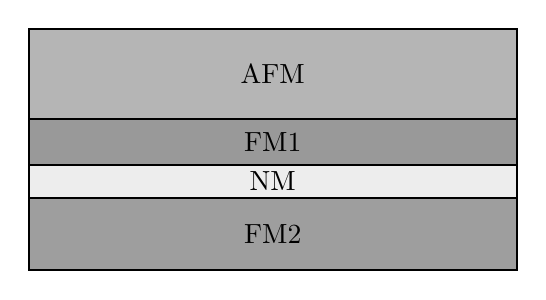
\begin{tikzpicture}[line width=0.8pt,>=Stealth]
\def\w{6.2}
% AFM (pinning layer, medium gray)
\fill[gray!58] (0,1.20) rectangle (\w,2.35);
\draw[line width=0.7] (0,1.20) rectangle (\w,2.35);
\node at (0.5*\w,1.775) {AFM};
% FM1 (darker gray)
\fill[gray!80] (0,0.62) rectangle (\w,1.20);
\draw[line width=0.7] (0,0.62) rectangle (\w,1.20);
\node at (0.5*\w,0.91) {FM1};
% NM spacer (brightest)
\fill[gray!14] (0,0.20) rectangle (\w,0.62);
\draw[line width=0.7] (0,0.20) rectangle (\w,0.62);
\node at (0.5*\w,0.41) {NM};
% FM2 (darker gray)
\fill[gray!76] (0,-0.72) rectangle (\w,0.20);
\draw[line width=0.7] (0,-0.72) rectangle (\w,0.20);
\node at (0.5*\w,-0.26) {FM2};
\end{tikzpicture}
\end{document}
